% !TeX spellcheck = fr_FR
\section{Validation du design}
Lors de cette section, sera décrite la procédure de vérification des caractéristiques du projet ainsi que sa validation.
\subsection{Liste de matériel} \label{ssec:ListeMateriel}
{
	\begin{enumerate}
		\item Oscilloscope Tektronix RTB2004 ES.SLO2.05.01.16 \label{enum:oscillo}
		\item Analyseur logique USB, 8 canaux, 24 MHz \label{enum:logicAnalyzer}
		\item USB vers TTL HW-597 \label{enum:USB-TTL}
		\item Carte Localisation-Sous-Marine V0.0 \label{enum:PCBL}
	\end{enumerate}
}

\subsection{Contrôle des alimentations}
{
	En premier lieu, une vérification des tensions d'alimentation permet de valider un aspect critique et fondamental de la carte.
	\subsubsection{Méthodologie}
	\paragraph{Mesure du 3.3V :} Alimentation de la carte par une connexion brève entre les pins du connecteur du bouton \textbf{P15}. Mesure sur le testpoint \textit{V\_regOUT5}, voir figure \ref{fig:sch3}.
	\begin{figure}[h]
		\centering
		\fbox{\includegraphics[width=0.3\linewidth]{Figures/DEV_MEAS/Sch3.3V}}
		\caption{Testpoint mesure 3.3V}
		\label{fig:sch3}
	\end{figure}
	
	\paragraph{Mesure du 5V :} Pour mesurer le 5V, il faut ponter par une résistance de $0\Omega$ la résistance R50, ainsi que activer la Pin RC5 / EN\_5V. Ensuite, la mesure a été prise sur le connecteur P16, pin-3, avec l'oscilloscope (Numéro \ref{enum:oscillo} de la liste de matériel \ref{ssec:ListeMateriel}) :
	\begin{figure}[h]
		\centering
		\fbox{\includegraphics[width=0.2\linewidth]{Figures/DEV_MEAS/Sch5V}}
		\caption{Schéma de mesure 5V}
		\label{fig:sch5v}
	\end{figure}
	
	\clearpage
	
	\subsubsection{Mesures}
	
	\begin{figure}
		\begin{subfigure}{.5\textwidth}
			\centering
			\includegraphics[width=\textwidth]{Mesures/Tension3.3V}
			\caption{Mesure 3.3V}
			\label{fig:Mes3.3V}
		\end{subfigure}
		\begin{subfigure}{.5\textwidth}
			\centering
			\includegraphics[width=\textwidth]{Mesures/Tension5V}
			\caption{Mesure 5V}
			\label{fig:Mes5V}
		\end{subfigure}
		\caption{Mesures des tensions d'alimentation}
		\label{fig:Mesure3.3et5V}
	\end{figure}
	
	\paragraph{Analyse :} Nous pouvons observer les valeurs respectives des tensions sur les figures \ref{fig:Mes3.3V} et \ref{fig:Mes5V}. La tension d'alimentation du microcontrôleur est mesurée à \textit{3.125V}, ce qui peut être expliqué par une chute de tension aux bornes de la batterie LI-ION qui nécessite donc d'être chargée. La tension 3.3V oscille légèrement, ce qui peut s'expliquer par le fait qu'il s'agit de l'alimentation principale de la carte avec le plus de consommateurs. Mais également par le fait que des signaux rapides sont générés par le microcontrôleur et ses différents périphériques.
	
	La tension d'alimentation du capteur de pression, dont la tension dimensionnée est de 5V, est quant à elle mesurée à \textit{5.0295V}, ce qui signifie une bonne précision de la part du circuit de boost. On peut également voir que la tension n'oscille pas et ne va donc pas perturber le capteur de pression.
	
	Nous pouvons donc confirmer le fonctionnement des blocs d'alimentation du projet.
}

\subsection{Communication UART}
{
	Comme décrit lors de la sous-section \ref{ssec:Usart}, une communication série est implémentée dans le projet. Cette communication n'est pas critique pour le projet, mais il est important de vérifier son fonctionnement pour d'éventuelles versions ultérieures.
	\subsubsection{Méthodologie}
	Pour la mesure, l'analyseur logique (Numéro \ref{enum:logicAnalyzer} de la liste de matériel \ref{ssec:ListeMateriel}) a été utilisé. Les trames U1TX et U1RX ont été mesurées sur le connecteur P4 :
	
	\begin{figure}[h]
		\centering
		\fbox{\includegraphics[width=0.2\linewidth]{Figures/DEV_MEAS/SchUart1}}
		\caption{Schéma de mesure UART1}
		\label{fig:schuart1}
	\end{figure}
	\clearpage	
	\subsubsection{Mesures}
	
	\begin{figure}[h]
		\centering
		\fbox{\includegraphics[width=1\linewidth]{Mesures/MesureTrameUart_Upscaled}}
		\caption{Mesures trames UART}
		\label{fig:mesuretrameuart}
	\end{figure}
	Nous pouvons lire des caractères ASCII sur la trame de la figure \ref{fig:mesuretrameuart}, qui reflètent le message envoyé contenant les mesures. 
	
	En connectant le module USB-TO-TTL (Numéro \ref{enum:USB-TTL} de la liste de matériel \ref{ssec:ListeMateriel}) aux broches Tx et Rx de la figure \ref{fig:mesuretrameuart}, puis en ouvrant une communication série via PuTTY à une baudrate de $115200$, nous obtenons la communication de la figure \ref{fig:puttytrames} dans la console :
	
	\begin{figure}[h]
		\centering
		\fbox{\includegraphics[width=0.65\linewidth]{Mesures/Putty_Trames}}
		\caption{Réception UART sur PuTTY}
		\label{fig:puttytrames}
	\end{figure}
	Analyse de la réception : Sur la figure \ref{fig:puttytrames}, on peut visualiser les données de la centrale inertielle, le temps écoulé entre chaque mesure, ainsi que les données du capteur de pression. Nous pouvons observer qu'entre chaque mesure, il s'écoule un laps de temps de $60 ms$, ce qui est plus rapide que les spécifications demandées par le cahier des charges. La mesure du capteur de pression à $-1.236$ bar n'est pas cohérente, car le capteur de pression n'était pas connecté au moment des mesures. Nous pouvons également constater que les mesures de la centrale inertielle sont cohérentes selon les données typiques d'une centrale inertielle\footnote{Exemple de données de fusion d'une centrale inertielle \cite{rozbicka2021estimation}}.
	
	\clearpage
}

\subsection{Communication SPI, carte SD}
{
	Il reste maintenant un élément critique à valider : la communication SPI avec la carte SD. Cette communication permet le logging des valeurs de mesure et est donc un aspect essentiel du projet.
	\subsubsection{Méthodologie}
	Pour cette mesure j'ai mesuré les signaux (SCK, SDO1, SDI1, CS\_SD) du SPI avec l'analyseur logique (Numéro \ref{enum:logicAnalyzer} de la liste de matériel \ref{ssec:ListeMateriel}).
	
	\begin{figure}[h]
		\centering
		\fbox{\includegraphics[width=0.35\linewidth]{Figures/DEV_MEAS/SchSpiSd}}
		\caption{Schéma de mesure carte SD}
		\label{fig:schspisd}
	\end{figure}
		
	\subsubsection{Mesures}
	\begin{figure}[h]
		\centering
		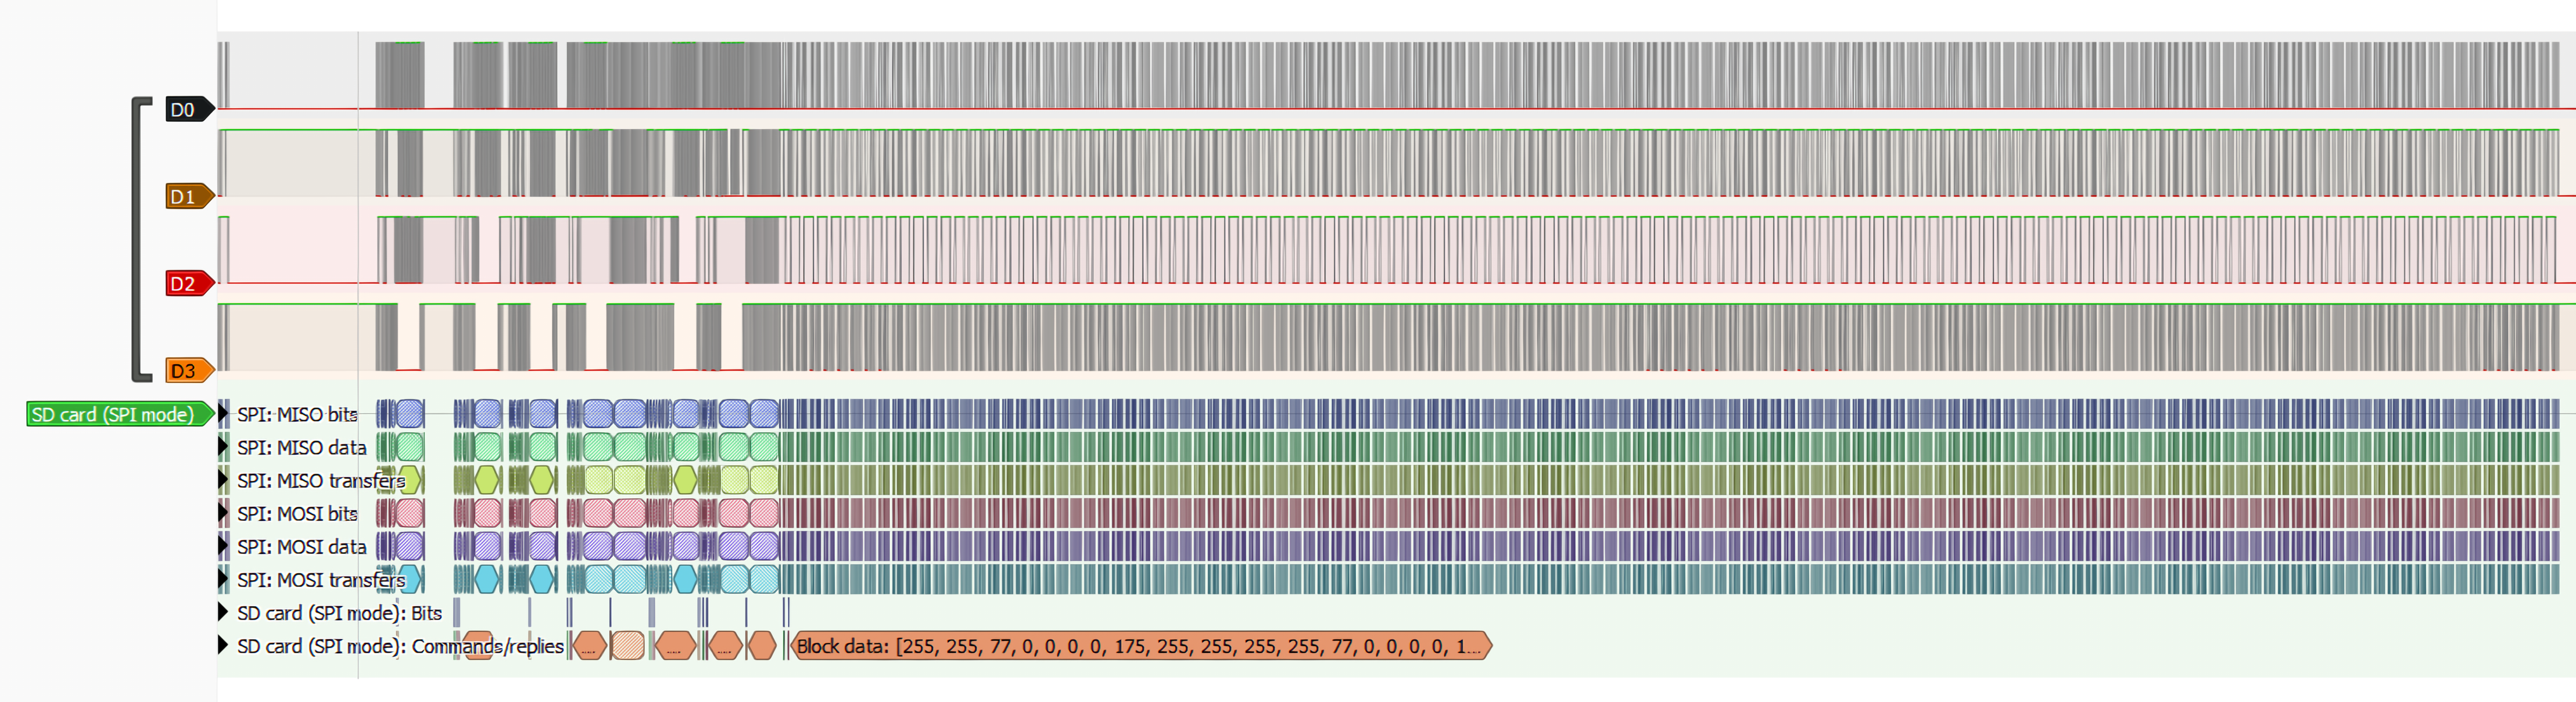
\includegraphics[width=1\linewidth]{Mesures/SPI_SD_CommEnsemble_Upscaled}
		\caption{Vue d'ensemble de la communication SPI}
		\label{fig:spisdcommensembleupscaled}
	\end{figure}
	Comme le montre la figure \ref{fig:spisdcommensembleupscaled}, on peut constater que les trames SPI utilisées pour la gestion de la FAT sont nombreuses. C'est pourquoi il est important d'avoir une fréquence élevée afin d'optimiser le temps des échanges de données.
	
	Nous allons maintenant mesurer le temps entre deux écritures sur la carte SD afin de vérifier le temps écoulé entre les mesures. et l'écriture.
	
	\clearpage
	
	\begin{figure}[h]
		\centering
		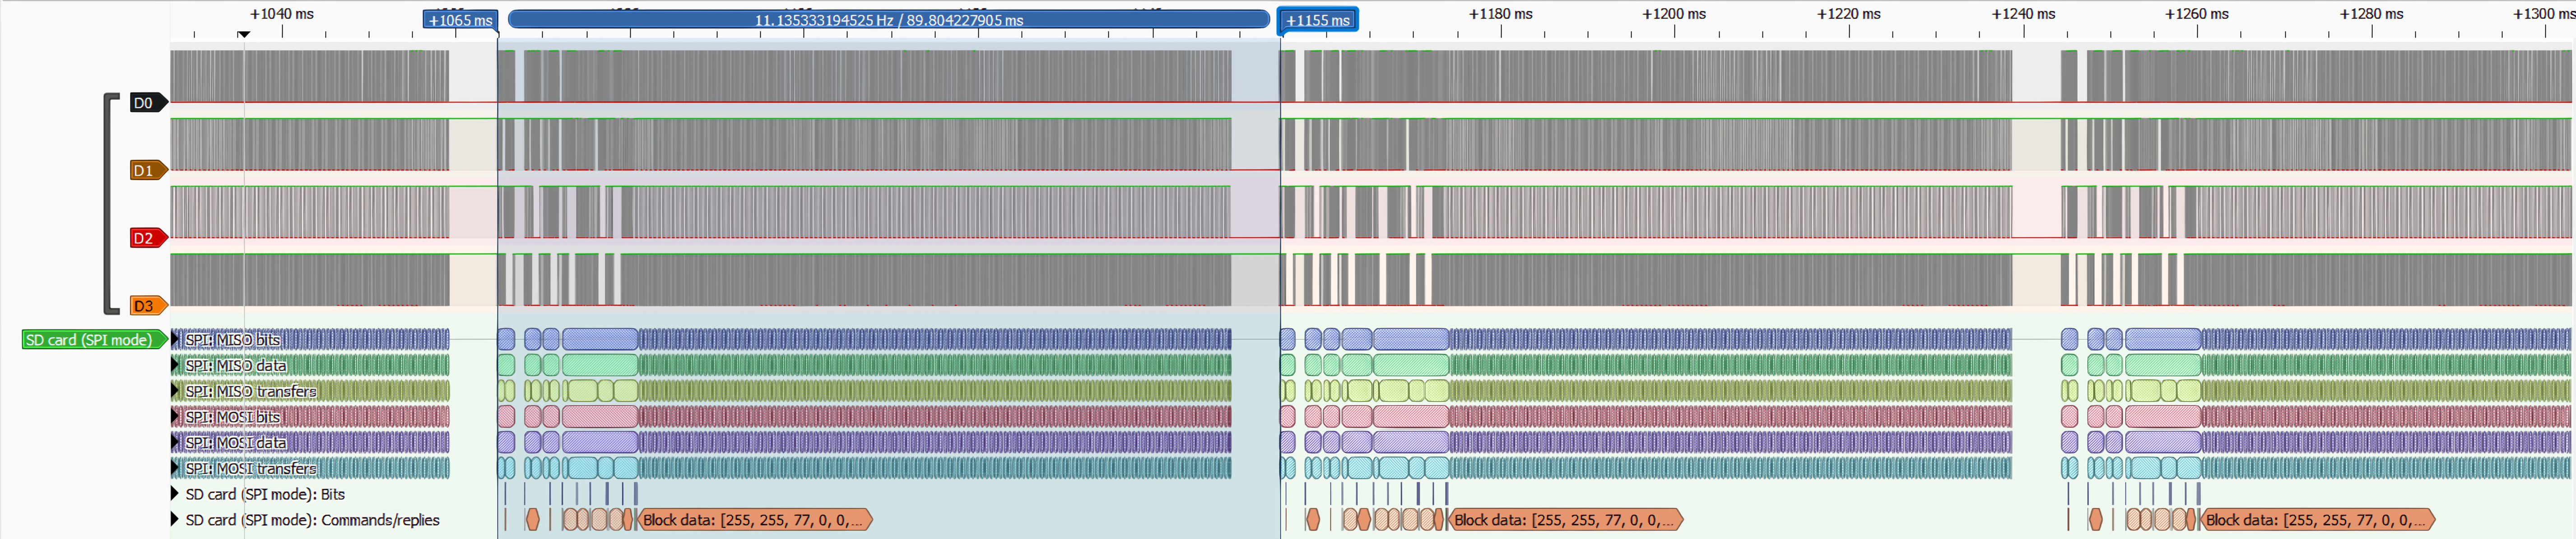
\includegraphics[width=1\linewidth]{Mesures/SPI_SD_TempreEntre2Comms_Upscaled}
		\caption{Temps entre deux écritures sur la carte SD}
		\label{fig:spisdtempreentre2commsupscaled}
	\end{figure}
	
	Nous pouvons observer sur la figure \ref{fig:spisdtempreentre2commsupscaled} que le temps mesuré entre une première écriture et le début de la suivante est de $89.804 ms$. Le temps disponible entre deux écritures est d'environ $\sim6ms$.
	Nous pouvons donc constater l'importance d'une vitesse élevée sur la communication SPI et sur le microcontrôleur.
	
	Avec une fréquence d'horloge de $48MHz$, on peut donc déduire :
	
	\begin{equation} 
		\label{equ:Noperations}
		N_{op} = T_{dispo} * F_{sys} = 6*10^{-3} * 48*10^{6} = 288'000 
	\end{equation}
	
	D'après le calcul \ref{equ:Noperations} nous savons que le MCU peut effectuer $288'000$ cycles machines durant ce temps disponible. Nous considérons ce nombre d'opérations suffisants au système, sachant qu'il n'y a pas beaucoup d'autre opérations. \textbf{Cet élément est à prendre en compte en cas d'ajout de fonctionnalité dans le système}.
	
	\paragraph{Mesure début de trame :} Sur la figure \ref{fig:spisdtramedepartupscaled} nous pouvons observer à quoi ressemble un début de trame sur la carte SD pour système FAT.
	
	\begin{figure}[h]
		\centering
		\includegraphics[width=1\linewidth]{Mesures/SPI_SD_Trame_Depart_Upscaled}
		\caption{Mesure début de trame}
		\label{fig:spisdtramedepartupscaled}
	\end{figure}
	
	
	
}

\clearpage

\section{Caractéristiques du produit fini}

% Please add the following required packages to your document preamble:
% \usepackage{graphicx}
\begin{table}[h]
	\centering
	\resizebox{\columnwidth}{!}{%
		\begin{tabular}{|l|rlrl|}
			\hline
			Caractéristique          & \multicolumn{2}{c|}{Attribut}                       & \multicolumn{2}{c|}{Valeur alternative} \\ \hline
			Axes de mesures          & $9$                 & \multicolumn{1}{l|}{}         & -                   &                   \\ \hline
			Mesures                  & \multicolumn{4}{c|}{$[ms][bar][\degree/s][uT][Euler][Quaternion][\degree C]$}                              \\ \hline
			Temps entre mesures      & $90$                & \multicolumn{1}{l|}{$[ms]$}   & $11.11$             & $Hz$              \\ \hline
			Nombre de mesures max    & $1.641$             & \multicolumn{1}{l|}{$M$}      & -                   &                   \\ \hline
			Capacité carte SD        & $256$               & \multicolumn{1}{l|}{$[MB]$}   & -                   &                   \\ \hline
			Pression maximum         & $10$                & \multicolumn{1}{l|}{$[bars]$} & $145$               & $PSI$             \\ \hline
			Autonomie                & $\sim20$            & \multicolumn{1}{l|}{$[h]$}    & $72'000$            & $[s]$             \\ \hline
			Batterie                 & $3400$              & \multicolumn{1}{l|}{$[mAh]$}  & $11.22$             & $[Wh]$            \\ \hline
			Profondeur               & $101.97$            & \multicolumn{1}{l|}{$[mH2O]$} & -                   &                   \\ \hline
			Précision pression       & $0.15$              & \multicolumn{1}{l|}{$[\%]$}    & -                   &                   \\ \hline
			Slot Mikroe              & $1$                 & \multicolumn{1}{l|}{$[-]$}    & -                   &                   \\ \hline
			Vitesse MCU              & $48$                & \multicolumn{1}{l|}{$[MHz]$}  & -                   &                   \\ \hline
			Interface                & LED RGB             & \multicolumn{1}{l|}{}         & -                   &                   \\ \hline
			Communications           & I2C, SPI, UART, USB & \multicolumn{1}{l|}{}         & -                   &                   \\ \hline
			Vitesse SPI              & $5$                 & \multicolumn{1}{l|}{$[MHz]$}  & -                   &                   \\ \hline
			Vitesse UART             & $115200$            & \multicolumn{1}{l|}{$[Bd]$}   & -                   &                   \\ \hline
			Mise en évidence mesure  & Oui                 & \multicolumn{1}{l|}{}         & -                   &                   \\ \hline
			Compensation température & Oui                 & \multicolumn{1}{l|}{}         & -                   &                   \\ \hline
		\end{tabular}%
	}
	\caption{Caractéristiques du projet V0.0}
	\label{tab:Caracteristiques}
\end{table}

On peut voir sur le tableau \ref{tab:Caracteristiques} les caractéristiques issues du développement final du projet dans sa version 0.0. Un test de logging de 5 heures a été effectué sans difficulté et a récolté 30 MB de données dans le fichier CSV, ce qui correspond effectivement aux caractéristiques du tableau \ref{tab:Caracteristiques}.